\documentclass{article}
\usepackage[pdftex]{graphicx} %for embedding images
\usepackage{url} %for proper url entries
\usepackage[bookmarks, colorlinks=false, pdfborder={0 0 0}, pdftitle={Introduction to Machine Learning Midterm}, pdfauthor={Nhut-Nam Le}, pdfsubject={troduction to Machine Learning}, pdfkeywords={report, exercises}]{hyperref} %for creating links in the pdf version and other additional pdf attributes, no effect on the printed document
%\usepackage[final]{pdfpages} %for embedding another pdf, remove if not required
\usepackage[utf8]{vietnam}
\usepackage{float}
\usepackage{fancyhdr}
\usepackage[utf8]{inputenc}
\usepackage{pythonhighlight}
\usepackage[left=3cm, right=3cm, top=2cm, bottom=2cm]{geometry}
\usepackage{parskip}
\usepackage{tikz}
\usepackage{hyperref}
\usepackage[]{algorithm2e}
\usepackage[noend]{algpseudocode}

\usepackage{listings}
\usepackage{color}

\definecolor{dkgreen}{rgb}{0,0.6,0}
\definecolor{gray}{rgb}{0.5,0.5,0.5}
\definecolor{mauve}{rgb}{0.58,0,0.82}

\newcommand\T{\rule{0pt}{2.6ex}}       % Top strut
\newcommand\B{\rule[-1.2ex]{0pt}{0pt}} % Bottom strut


\newcommand{\foo}{\hspace{-2.3pt}$\bullet$ \hspace{5pt}}


\lstset{frame=tb,
	language=Java,
	aboveskip=3mm,
	belowskip=3mm,
	showstringspaces=false,
	columns=flexible,
	basicstyle={\small\ttfamily},
	numbers=none,
	numberstyle=\tiny\color{gray},
	keywordstyle=\color{blue},
	commentstyle=\color{dkgreen},
	stringstyle=\color{mauve},
	breaklines=true,
	breakatwhitespace=true,
	tabsize=3
}

\setlength{\parindent}{15pt}
\setlength{\headheight}{15.2pt}
\pagestyle{fancy}
\lhead[<even output>]{Nhập môn Học Máy}
\rhead[<even output>]{Báo cáo Giữa kỳ}
\title{research-outline}
\author{Nhut-Nam Le}
\date{2021}

\begin{document}
	\begin{titlepage}
		\begin{center}
			% Top of the page
			\large{\textbf{ĐẠI HỌC KHOA HỌC TỰ NHIÊN, ĐHQG-HCM\\KHOA CÔNG NGHỆ THÔNG TIN\\BỘ MÔN KHOA HỌC MÁY TÍNH}}\\
			
\includegraphics[width=0.75\textwidth]{images/khtn.png}\\
			% Title
			\large \textbf{NHẬP MÔN HỌC MÁY}\\[0.1in]
			\huge \textbf{BÁO CÁO ĐỒ ÁN GIỮA KỲ}\\[0.1in]
			\huge \textbf{TÌM HIỂU: NHẬN DẠNG GIỌNG NÓI BẰNG SÓNG ÂM THÔ VỚI SINCNET}\\[0.1in]
			\vfill
			\normalsize
			\normalsize
			% Lecturers
			\textbf{Giảng viên lý thuyết}\\
			{\textbf{TS.} Bùi Tiến Lên}\\[0.1in]
			% Teacher Assistant
			\textbf{Giảng viên hướng dẫn}\\
			\vspace{0.1in}
			{Dương Nguyễn Thái Bảo, Nguyễn Ngọc Đức, Nguyễn Tiến Huy, Lê Thanh Phong}\\[0.1in]
			\textbf{Sinh viên thực hiện} \\
			\vspace{0.1in}
			% Submitted by
			{Vương Gia Bảo, Ngô Xuân Kiên, Lê Nhựt Nam, Nguyễn Viết Dũng}\\[0.1in]
			% Date time when written report
			\vfill
			Tháng 4 năm 2021
		\end{center}
	\end{titlepage}
	\newpage
	% End Title4
	
	\pagenumbering{roman} %numbering before main content starts
	\cleardoublepage
	%\pagebreak
	\phantomsection
	\addcontentsline{toc}{section}{Lời cảm ơn}
	\section*{Lời cảm ơn}
	\vspace{1.0in}
	\begingroup
	\setlength{\parindent}{0pt}
	\qquad Trong quá trình thực hiện đồ án này, chúng em đã nhận được rất nhiều sự giúp đỡ cũng như hỗ trợ từ các thầy cô Trường Đại học Khoa học Tự nhiên, ĐHQG-HCM và các bạn bè trong lớp Nhập môn Học Máy. Em xin bày tỏ lòng cảm ơn chân thành đến mọi người vì đã giúp đỡ hướng dẫn, chỉ bảo rất tận tình.
	
	\qquad Đặc biệt, em xin bày tỏ lòng biết ơn sâu sắc đến các thầy cô khoa Công nghệ Thông tin, cụ thể hơn là thầy Bùi Tiến Lên và các thầy hướng dẫn đã giảng dạy rất nhiệt, cung cấp nhiều slides, tài nguyên học tập cần thiết, tạo điều kiện tốt nhất để bản thân em có thể hoàn thành được đồ án này.
		
	\qquad Trong quá trình, viết báo cáo này, bản thân em không thể tránh khỏi nhiều sai sót về mặt chuyên môn phân tích thuật toán, đọc hiểu và dịch thuật các từ tiếng Anh chuyên ngành Khoa học Máy tính. Em mong nhận được góp ý để hoàn thiện hơn đối với đồ án này, cũng như rút kinh nghiệm cho những đồ án, những báo cáo kế tiếp.
	
	\vspace{1.0in}
	\textbf{Đại học Khoa học Tự nhiên, ĐHQG-HCM.}\\
	Lê Nhựt Nam\\
	Tháng 4 năm 2021\\
	\endgroup
	
	\newpage
	\tableofcontents
	\newpage
	\pagenumbering{arabic} %reset numbering to normal for the main content
	\setcounter{secnumdepth}{0}
	
	\section{1. Đặt vấn đề}
	
	Trong những năm gần đây, Machine Learning (Học máy/ Máy học) đạt được rất nhiều thành tựu nổi bật, thúc đẩy Cách mạng Công nghệ 4.0 phát triển nhanh chóng. Một trong những tác nhân chính mạnh mẽ nhất đến từ Deep Learning (Deep Neural Networks - Các mạng Học sâu), các mô hình học dựa trên những phương pháp này đã rất thành công, đạt được một hiệu năng đầy triển vọng, trong nhiều tác vụ khác nhau như Thị giác Máy tính (Computer Vision), Nhận dạng Nhân trắc học (Biometrics): Giọng nói (Speech), Khuôn mặt (Face), Vân tay (Fingerprint), ..., Xử lý ngôn ngữ tự nhiên (Natural Language Processing), ...
	
	Trong tác vụ nhận dạng, đặc biệt là nhận dạng giọng nói (Voice/ Speech Recognition) gần như là một bài toán khó trong nhiều năm, cần những phương pháp rất phức tạp để có thể giải quyết được. Nhờ vào Học sâu, phương giải phải khả thi, mà cụ thể là với Mạng Neural Tích chập (Convolutional Neural Networks - CNNs) đem lại những kết quả đầy hứa hẹn khi chỉ cần đầu vào trực tiếp là mẫu giọng nói thô. Thay vì sử dụng các tính năng thủ công tiêu chuẩn, CNNs sau này học cách biểu diễn giọng nói cấp thấp từ các dạng sóng, có khả năng cho phép mạng nắm bắt tốt hơn các đặc điểm loa dải hẹp quan trọng như cao độ và định dạng.
	
	Với mục đích tìm hiểu bài báo khoa học, cũng như tìm hiểu những mô hình, phương pháp Học máy nổi bật gần đây trong những tác vụ quan trọng, mà cụ thể là nhận dạng. Nhóm chúng em quyết định chọn một bài báo khoa học làm tài liệu thực hiện chính cho đồ án môn học
	
	Thông tin bài báo
	\begin{itemize}
		\item Tên bài báo: Speaker Recognition from Raw Waveform with SincNet
		
		\item Tác giả: Mirco Ravanelli và Yoshua Bengio
		
		\item Năm công bố: 2019
		
		\item eprint: 1808.00158
		
		\item archivePrefix: arXiv
		
		\item primaryClass: eess.AS
		
		\item Source code chính thức: \href{https://github.com/mravanelli/SincNet}{https://github.com/mravanelli/SincNet}
	\end{itemize}

	\section{2. Động lực nghiên cứu khoa học}
	\qquad Tính phổ biến của tín hiệu giọng nói, phạm vi ứng dụng có thể có của sinh trắc học (nhân trắc học) giọng nói rộng hơn so với các đặc điểm sinh trắc học thông thường khác. Chúng ta có thể phân biệt ba loại ứng dụng chính tận dụng thông tin sinh trắc học có trong tín hiệu giọng nói như sau:
	\begin{itemize}
		\item \textbf{Voice authentication (Xác nhận giọng nói)} (Access control - Điều khiển truy cập, thường là điều khiển từ xa bằng điện thoại) và back-ground recognition (Nhận dạng lý lịch) (natural voice checking - kiểm tra bằng giọng nói tự nhiên).
		\item \textbf{Speaker detection (Nhận diện người nói)} (ví dụ như: phát hiện danh sách đen trong các tổng đài điện thoại hoặc trong nghe lén và giám sát, …), hay còn được gọi là speaker spotting
		\item \textbf{Forensic speaker recognition (Nhận dạng người nói trong Pháp y)} (sử dụng giọng nói làm bằng chứng trước tòa án hoặc làm thông tin tình báo trong các cuộc điều tra của cảnh sát hình sự) 
	\end{itemize}
	\qquad Các phương pháp SOTA dựa trên việc biểu diễn i-vectors của những đoạn giọng nói, cải thiện đáng kể so với mô hình Gaussian Mixture Model-Universal Background Models và sự phát triển của Deep Neural Network đã góp phần giải quyết nhận dạng giọng nói. Tuy nhiên vẫn còn nhiều vấn đề cần phải giải quyết với bài toán này như vấn đề dữ liệu đầu vào, tối ưu độ lỗi, tăng hiệu năng hội tụ và nhất là làm sao thiết kế một mô hình nhỏ gọn, có thể tinh chỉnh được để phù hợp với các ứng dụng của chúng ta.
	
	\section{3. Phát biểu bài toán}
	
	\textbf{Tác vụ:} Định danh người nói
	\begin{itemize}
		\item Đầu vào (Input): Dữ liệu âm thanh giọng nói
		\item Đầu ra (Output): Danh tính của người nói
	\end{itemize}
	\textbf{Tác vụ:} Xác nhận người nói
	\begin{itemize}
		\item Đầu vào (Input): Dữ liệu âm thanh giọng nói
		\item Đầu ra (Output): Đồng ý/ Từ chối
	\end{itemize}
	
	\section{4. Phương pháp tiếp cận của nhóm}
	\begin{itemize}
		\item Tìm hiểu ý tưởng chính, kiến trúc mạng SincNet, phương pháp được tác giả đề cập trong bài báo.
		\item Tóm tắt, diễn giải, chứng minh công thức đã tìm hiểu từ bài báo.
		\item Tìm hiểu cách xử lý dữ liệu, xây dựng mô hình, huấn luyện mô hình, đánh giá mô hình từ source code chính thức của tác giả bài báo.
		\item Tìm hiểu, thu thập, xây dựng dữ liệu.
		\item Chỉnh sửa source code của tác giả cho phù hợp với phần cứng, phần mềm hiện tại mà nhóm có, huấn luyện mô hình, đánh giá mô hình, trình bày kết quả đạt được.
		\item Trình bày những gì tìm hiểu, làm được thông qua Video Clip.
	\end{itemize}

	\section{3. Trình bày lại nội dung bài báo}
	
	\subsection{3.1 Giới thiệu về bài báo}
	
	\qquad Nhóm tác giả trong bài báo này đề xuất một kiến trúc mạng CNN (Convolutional Neural Networks) mới, được gọi là SincNet, khai phá lớp tích chập đầu tiên để khám phá nhiều thông tin hơn. SincNet dựa trên các hàm $sinc$ được tham số hóa, để cài đặt các bộ lọc băng thông.
	
	Ngược lại với CNNs chuẩn, học tất cả các phần tử của mỗi bộ lọc filter, ở đây, chúng ta chỉ có các tần số cắt thấp và cao học trực tiếp dữ liệu với phương pháp đề xuất
	
	Cung cấp một tập các bộ lọc mà chúng nhỏ gọn và hiệu quả trong việc tùy chỉnh với ứng dụng mà chúng ta muốn.
	
	Đây là một sự kết hợp tuyệt vời giữa Học máy (Machine Learning) và Xử lý Tín hiệu số (Digital Signal Processing)
	
	Bài báo được đăng công khai trên \href{arxiv.org}{arXiv dot org} lần đầu tiên vào năm 2018 bởi hai người Mirco Ravanelli, Yoshua Bengio (ông được xem là một trong 3 vị cha đẻ của phương pháp Deep Learning hiện đại), phiên bản cập nhật gần đây nhất là vào năm 2019 bằng việc thay thế hàm "sinc\_conv" bằng "SincConv\_fast" giúp tăng tốc độ lên 50\% so với phiên bản cũ.
	
	\subsubsection{3.1.1 Về nhận dạng giọng nói}
	\qquad Về lĩnh vực Nhận dạng giọng nói, đây là một lĩnh vực nghiên cứu có nhiều ứng dụng vào thực tiễn đời sống như xác thực sinh trắc học, pháp y, bảo mật, nhận dạng giọng nói và phân cực giọng nói.
	
	Hầu hết những giải pháp "state of the art" đều dựa trên việc biểu diễn \textbf{i-vectors} của những đoạn giọng nói, cải thiện đáng kể so với mô hình Gaussian Mixture Model-Universal Background Models (GMM-UBMs).
	
	Trong những năm gần đây, Trí tuệ Nhân tạo nhất là lĩnh vực Học máy (Machine Learning) đạt được nhiều thành tựu nổi bật là nhờ Học Sâu (Deep Learning). Các mạng học sâu - Deep Neural Networks (DNNs) sử dụng trong những framework i-vector để tính toán thống kê Baum-Welch hoặc trong các khung rút trích đặc trưng theo mức (frame-level feature extraction). Ngoài ra, DNNs còn được dùng trong việc phân tách giọng nói.
	
	Những kỹ thuật này cần phải tuân theo một số tiêu chuẩn nhất định, ví dụ như: độ mượt của tần số giọng nói có thể làm cản trở việc rút trích một số đặc trưng của giọng nói như cao độ và ngữ âm, .... Để khắc phục chúng, các công trình mới đây thường dùng kỹ thuật spectrogram bins (bin tần số) hoặc dùng cả sóng thô (raw waveform).
	
	\subsubsection{3.1.2 Về Convolutional Neural Networks}
	\qquad Convolutional Neural Networks - CNNs là một lựa chọn thích hợp với đầu vào là những sóng thô, nó kiến trúc phổ biến nhất để xử lý các mẫu giọng nói thô nhờ vào chia sẻ trọng số, bộ lọc cục bộ và tổng hợp giúp khám phá các biểu diễn dữ liệu và bất biến.
	
	Vấn đề lớn nhất đối với sóng thô dựa trên mạng CNNs chính là \textbf{lớp tích chập đầu tiên}.
	\begin{figure}[H]
		\centering
		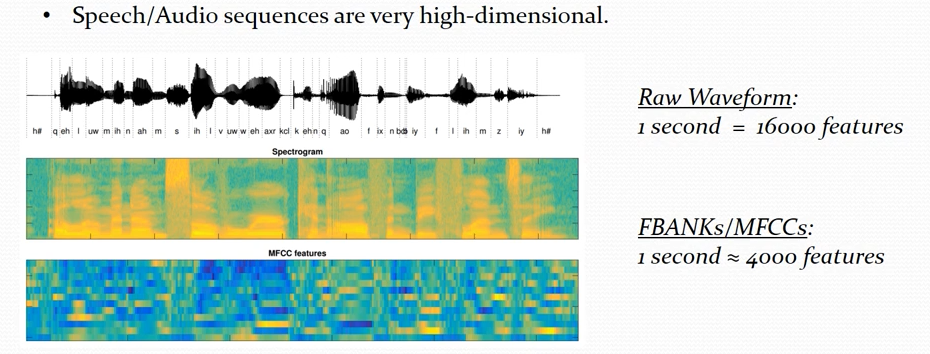
\includegraphics[width=1\textwidth]{images/capture_01.png}
		\caption{Minh họa chuỗi giọng nói có số chiều rất lớn. Ảnh được lấy từ video A bref introduction to SincNet thực hiện bởi Giáo sư Mirco Ravanelli}
		\label{fig:writing-thesis}
	\end{figure}
	Ở lớp này, dữ liệu đầu vào là những chuỗi Speech/Audio có số chiều rất cao, ví dụ như: cứ mỗi giây thì ta lại có đến 16000 đặc trưng. Bằng những kỹ thuật "bằng tay" ngày xưa như FBANKs hay MFCCs thì ta có thể giúp nó giảm xuống còn 4000 đặc trưng mỗi giây, nhưng như thế vẫn còn rất nhiều!
	
	Những đặc trưng trong phổ tần số có thể nhận ra bằng mắt thường nhưng lại bị mất đi nếu chúng ta làm mịn chúng.
	\begin{figure}[H]
		\centering
		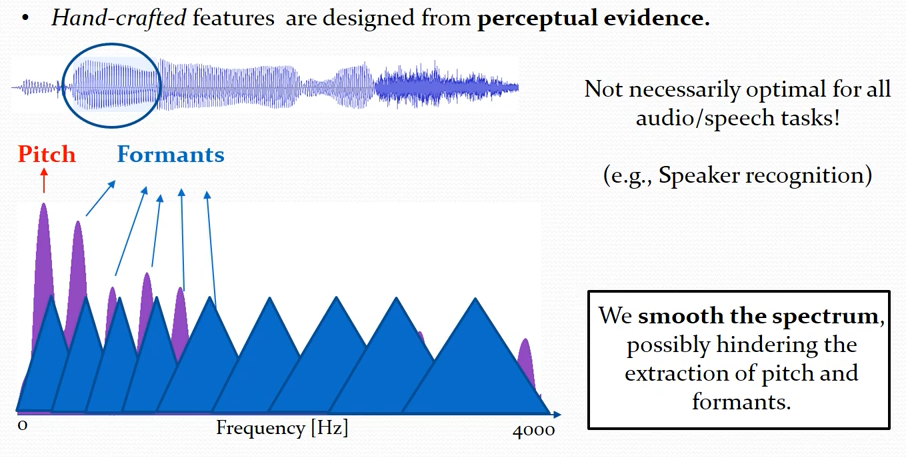
\includegraphics[width=1\textwidth]{images/perceptual_evidence.png}
		\caption{Ảnh được lấy từ video A bref introduction to SincNet thực hiện bởi Giáo sư Mirco Ravanelli}
		\label{fig:writing-thesis}
	\end{figure}
	
	Không những gặp vấn đề về số chiều dữ liệu mà còn bị ảnh hưởng nhiều hơn bởi các vấn đề về sự biến mất độ dốc đạo hàm, đặc biệt là khi sử dụng các kiến trúc rất sâu.
	\begin{figure}[H]
		\centering
		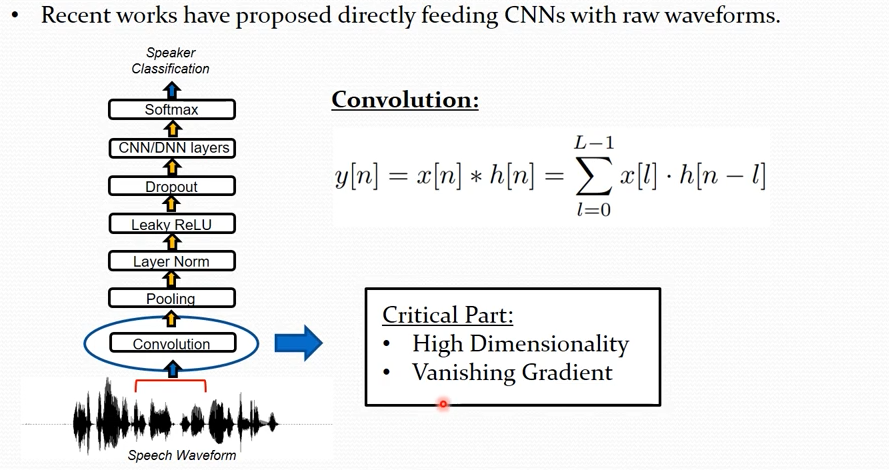
\includegraphics[width=1\textwidth]{images/cnns_problems.png}
		\caption{Ảnh được lấy từ video A bref introduction to SincNet thực hiện bởi Giáo sư Mirco Ravanelli}
		\label{fig:writing-thesis}
	\end{figure}
	
	Các bộ lọc CNNs thường có những hình dạng đa băng tần không hợp lý, để hiểu nó thì với mạng Neural là điều dễ dàng, nhưng với con người thì nó không có nhiều ý nghĩa trong việc thể hiện giọng nói.
	\begin{figure}[H]
		\centering
		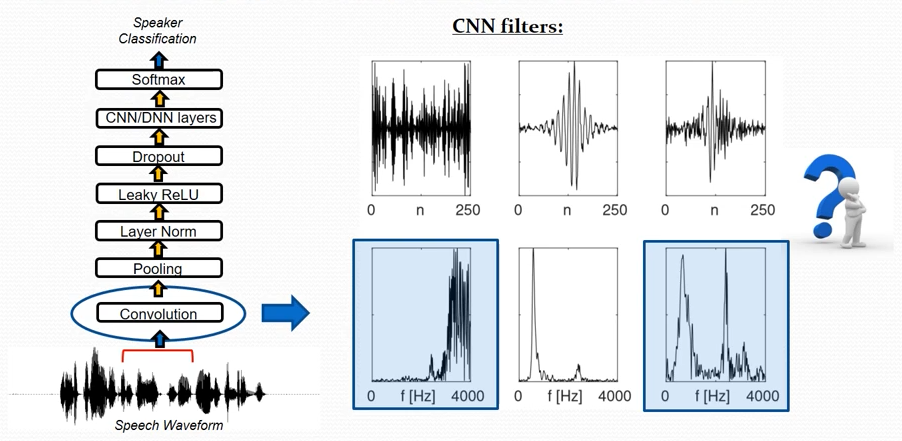
\includegraphics[width=1\textwidth]{images/interpretability_problems.png}
		\caption{Ảnh được lấy từ video A bref introduction to SincNet thực hiện bởi Giáo sư Mirco Ravanelli}
		\label{fig:writing-thesis}
	\end{figure}
	
	
	\subsection{3.2 Kiến trúc mạng SincNet}
	
	Với một CNN chuẩn, việc tích chập trong miền thời gian giữa input waveform và một số đáp ứng xung hữu hạn (Finite Impulse Response - FIR) được cho bởi công thức:
	
	$$y[n] = x[n] * h[n] = \sum_{l=0}^{L-1}x[l].h[n-l]$$ 
	
	Trong đó:
	\begin{itemize}
		\item $x[n]$: đoạn tín hiệu giọng nói
		\item $h[n]$: một mặt nạ ứng với chiều dài $L$
		\item $y[n]$: giá trị đầu ra
	\end{itemize}
	
	Trong khi đó, Sincnet thực hiện các phép tích chập của nó với hàm $g$, hàm này phụ thuộc vào một tham số $\theta$. Công thức như sau:
	
	$$y[n] = x[n] * g[n, \theta]$$
	
	Trong xử lý tín hiệu số, $g$ được định nghĩa như một filter-bank gồm các bộ lọc (filter) băng thông hình chữ nhật. Trong miền tần số, độ lớn của một bộ lọc băng thông tổng quát có thể được tính như hiệu số giữa 2 bộ lọc thông tần số thấp
	
	Với $f_1$ $f_2$ lần lượt là tần số cắt thấp (low) và cao (high) đã được học, $rect(.)$ là hàm rectangular trong miền tần số.
	
	$$G[f, f_1, f_2] = rect\left(\frac{f}{2f_2}\right) -  rect\left(\frac{f}{2f_1}\right)$$
	
	Công thức trên đang ở trong miền tần số, để có thể trở lại miền thời gian được, ta sử dụng phép biến đổi Fourier Ngược
	
	Note: Biến đổi Fourier cho hàm Rectangular
	
	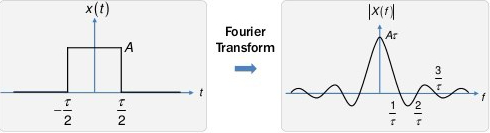
\includegraphics[width=1\textwidth]{images/rect_fourier.jpg}\\
	
	$$x(t) = Arect(\frac{t}{\tau})$$
	
	Biến đổi:
	
	$$X(\omega) = \int_{-\infty}^{\infty} x(t)e^{-j \omega t}\;\mathrm{d}t 
	$$
	
	$$X(\omega) = \int_{-\frac{\tau}{2}}^{\frac{\tau}{2}} Ae^{-j \omega t}\;\mathrm{d}t 
	= -\frac{2A}{\omega}\left[\frac{e^{-\frac{j \omega \tau}{2}} - e^{\frac{j \omega \tau}{2}}}{2j}\right]
	= \frac{2A}{\omega} \left[sin\left(\frac{\omega \tau}{2}\right)\right]
	= A\tau \left[\frac{sin(\frac{\omega \tau}{2})}{\frac{\omega \tau}{2}}\right]
	$$
	
	Hàm $sinc$ được định nghĩa
	
	$$sinc(x) = \frac{sin(x)}{x}$$
	
	Theo đó:
	
	$$X(\omega) = A\tau sinc\left(\frac{\omega \tau}{2}\right)$$
	
	Áp dụng công thức:
	
	Biến đổi ngược:
	
	$$G[f, f_1, f_2] = rect\left(\frac{f}{2f_2}\right) -  rect\left(\frac{f}{2f_1}\right)$$
	
	Ta được hàm tham chiếu $g$
	
	$$g[n, f_1, f_2] = 2f_2sinc(2\pi f_2 n) - 2f_1sinc(2\pi f_1 n)$$ 
	
	Các tần số cắt (cut-off frequencies) có thể được khởi tạo một cách ngẫu nhiên trong khoảng $\left[0, \frac{f_2}{2}\right]$, trong đó $f_s$ là tần số mẫu của tín hiệu đầu vào.
	
	Tần suất lấy mẫu có thể thay đổi theo loại dữ liệu chúng ta đang thử nghiệm. Hệ thống IVR có tần số lấy mẫu là 8Khz, trong khi hệ thống âm thanh nổi có tần số lấy mẫu là 44khz.
	
	Chúng ta có thể khởi tạo các bộ lọc dựa trên các tần số cắt của bộ lọc mel-scale filter-bank. Ưu điểm chính của việc chỉ định bộ lọc theo cách này là nó có lợi thế là phân bổ trực tiếp nhiều bộ lọc hơn ở phần dưới của phổ có thông tin duy nhất về giọng nói của người nói.
	
	Để đảm bảo $f1 \geq 0$ và $f_2 \geq f_1$, phương trình phía trên được cung cấp bởi các tham số sau:
	
	$$f_{1}^{abs} = |f_1|$$
	
	$$f_{2}^{abs} = f_1 + |f_2 - f_1| $$
	
	Ở đây, không có giới hạn nào đối với $f_2$, tức là không có tác nhân nào tác động lên $f_2$ để nó có thể nhỏ hơn tần số Nyquist (tốc độ tối thiểu mà tín hiệu có thể được lấy mẫu mà không có lỗi, gấp đôi tần số cao nhất hiện có trong tín hiệu) như mô hình học điều này trong khi huấn luyện. Các lớp tiếp theo khác nhau quyết định mức độ quan trọng nhiều hơn hoặc ít hơn cho mỗi đầu ra bộ lọc.
	
	Bộ lọc băng thông lý tưởng cần có vô số phần tử $L$. Một bộ lọc băng thông lý tưởng là nơi băng thông hoàn toàn phẳng và độ suy giảm trong băng thông dừng là vô hạn. Bất kỳ sự cắt ngắn nào của $g$ chắc chắn dẫn sẽ đến sự xấp xỉ của bộ lọc lý tưởng, được đặc trưng bởi các gợn sóng trong băng thông và suy giảm giới hạn dừng băng thông.
	
	Vì vậy, giải pháp cửa sổ (windowing) được thực hiện để giải quyết vấn đề này. Nó được thực hiện chỉ bằng cách nhân hàm bị cắt ngắn $g$ với cửa sổ $w$, nhằm mục đích làm phẳng các điểm gián đoạn đột ngột ở cuối $g$
	
	$$g_{w}\left[n, f_1, f_2\right] = g[n, f_1, f_2 . w[n]$$
	
	Trong bài báo, tác giả sử dụng Hamming Window, được định nghĩa bởi công thức:
	
	$$w[n] = 0.54 - 0.46.cos(\frac{2\pi n}{L})$$
	
	
	Chúng ta có thể có được tính chọn lọc tần số cao với việc sử dụng cửa sổ Hamming. Chúng ta cũng có thể sử dụng các cửa sổ khác như Hann, Blackman, Kaiser window. Một lưu ý quan trọng ở đây là do tính đối xứng, các bộ lọc có thể được tính toán hiệu quả bằng cách xem xét một nửa bộ lọc và kế thừa kết quả cho nửa còn lại.
	
	Tần số cắt của các bộ lọc có thể được tối ưu với các thông số CNN sử dụng Stochastic Gradient Descent (SGD) hoặc các phương pháp tối ưu Gradient khác. Như mô hình bên dưới, CNN pipeline (Pooling, Normalization, Activations, Dropout) có thể được sử dụng sau tích chập dựa trên Sinc Convolution đầu tiên. Multiple standard convolutional, fully-connehoặccted hoặc recurrent layers có thể đặt chồng lên ở giai đoạn sau đó để cuối cùng qua Softmax Classifier (Bộ phân lớp Softmax) để phân lớp giọng nói.
	
	\begin{figure}[H]
		\centering
		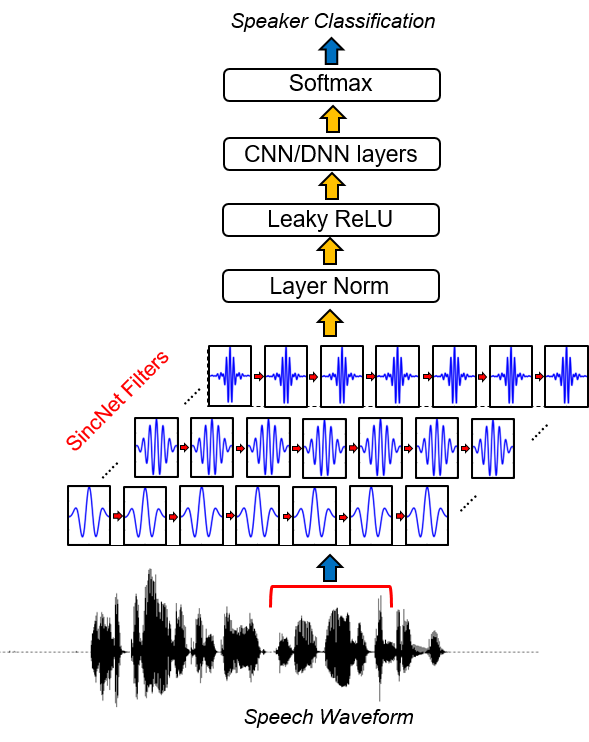
\includegraphics[width=1\textwidth]{charts/SincNet.png}
		\caption{Kiến trúc mạng Sicnet}
		\label{fig:writing-thesis}
	\end{figure}

	
	\textbf{Đặc điểm của mô hình mạng SincNet}
	\begin{itemize}
		\item \textbf{Tính hội tụ nhanh}
		\begin{itemize}
			\item Sincnet được thiết kế theo cách mà nó buộc mạng phải tập trung vào các thông số lọc ảnh hưởng đến tốc độ của nó. Phong cách kỹ thuật lọc này giúp thích ứng với dữ liệu trong khi nắm bắt được tri thức giống như kỹ thuật trích xuất đặc trưng trên dữ liệu âm thanh. Tiền tri thức này làm cho việc học các đặc tính của bộ lọc dễ dàng hơn nhiều, giúp SincNet hội tụ nhanh hơn đáng kể đến một giải pháp tốt hơn. Chúng ta có được sự hội tụ nhanh chóng trong vòng 10–15 epochs đầu tiên.
			\begin{figure}[H]
				\centering
				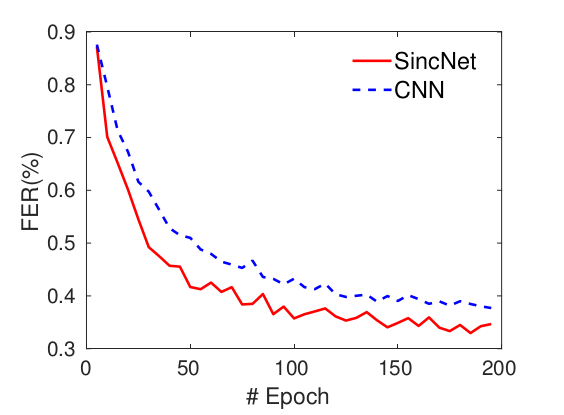
\includegraphics[width=0.5\textwidth]{images/fast_convergence.png}
				\caption{Độ hội tụ của SincNet so với CNN}
				\label{fig:writing-thesis}
			\end{figure}
		\end{itemize}
		\item \textbf{Tính hiệu quả}
		\begin{itemize}
			\item Do các hàm kernel $g(.)$ là đối xứng nên ta có thể thực hiện phép tích chập trên một phần filter và kế thừa kết quả này trên phần còn lại. Điều này sẽ tiết kiệm 50\% việc tính toán.
			\begin{figure}[H]
				\centering
				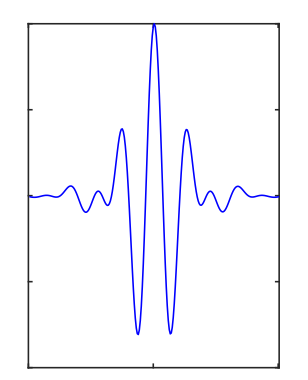
\includegraphics[width=0.3\textwidth]{images/g_symmetric.png}
				\caption{Hàm kernel}
				\label{fig:writing-thesis}
			\end{figure}
		\end{itemize}
		\item \textbf{Cần ít tham số cho việc huấn luyện mô hình}
		\begin{itemize}
			\item SincNet giảm đáng kể số lượng tham số trong lớp chập đầu tiên. Ví dụ: nếu chúng ta xem xét một lớp bao gồm các bộ lọc $F$ có độ dài $L$, một CNN tiêu chuẩn sử dụng các tham số $F * L$, so với $2F$ được SincNet xem xét. Nếu $F = 90$ và $L = 100$, chúng ta sử dụng $9000$ tham số cho CNN và chỉ $180$ cho SincNet. Hơn nữa, nếu chúng ta tăng gấp đôi độ dài bộ lọc $L$, một CNN chuẩn sẽ tăng gấp đôi số lượng tham số của nó (ví dụ: chúng ta đi từ $9000$ lên $18000$), trong khi SincNet có số lượng tham số không thay đổi (chỉ có hai tham số được sử dụng cho mỗi bộ lọc, bất kể độ dài $L$ của nó). Điều này cung cấp khả năng tạo ra các bộ lọc rất chọn lọc với nhiều lần nhấn, mà không thực sự thêm các tham số vào vấn đề tối ưu hóa. Hơn nữa, sự nhỏ gọn của kiến trúc SincNet làm cho nó phù hợp trong trường hợp ít mẫu.
		\end{itemize}
		\item \textbf{Tính giải nghĩa/ diễn giải}
		\begin{itemize}
			\item Các feature maps của SincNet sau khi thực hiện lớp tích chập đầu tiên rất dễ hiểu và con người có thể hiểu được so với những cách tiếp cận khác. Trên thực tế, các filter-bank chỉ phụ thuộc vào các tham số có ý nghĩa vật lý rõ ràng.
		\end{itemize}
		\begin{figure}[H]
			\centering
			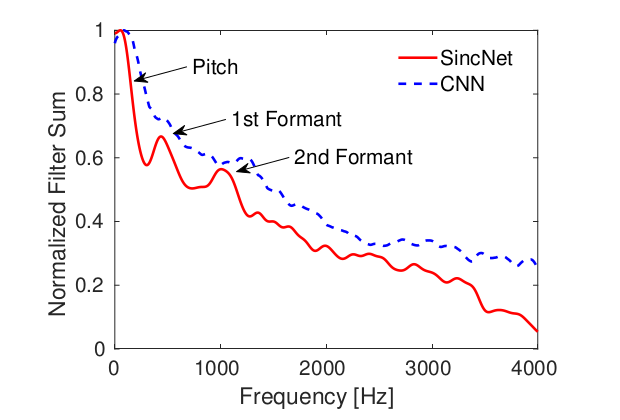
\includegraphics[width=0.5\textwidth]{images/interpretability.png}
			\caption{Khả năng diễn giải của SincNet so với CNN}
			\label{fig:writing-thesis}
		\end{figure}
	
		\begin{figure}[H]
			\centering
			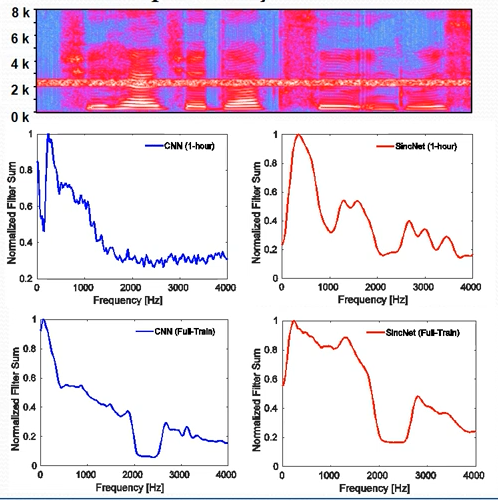
\includegraphics[width=0.85\textwidth]{images/interpretability_2.png}
			\caption{Khả năng diễn giải của SincNet so với CNN}
			\label{fig:writing-thesis}
		\end{figure}
	\end{itemize}

	\textbf{Đối chiếu Convolution Neural Networks với SincNet}
	\begin{figure}[H]
		\centering
		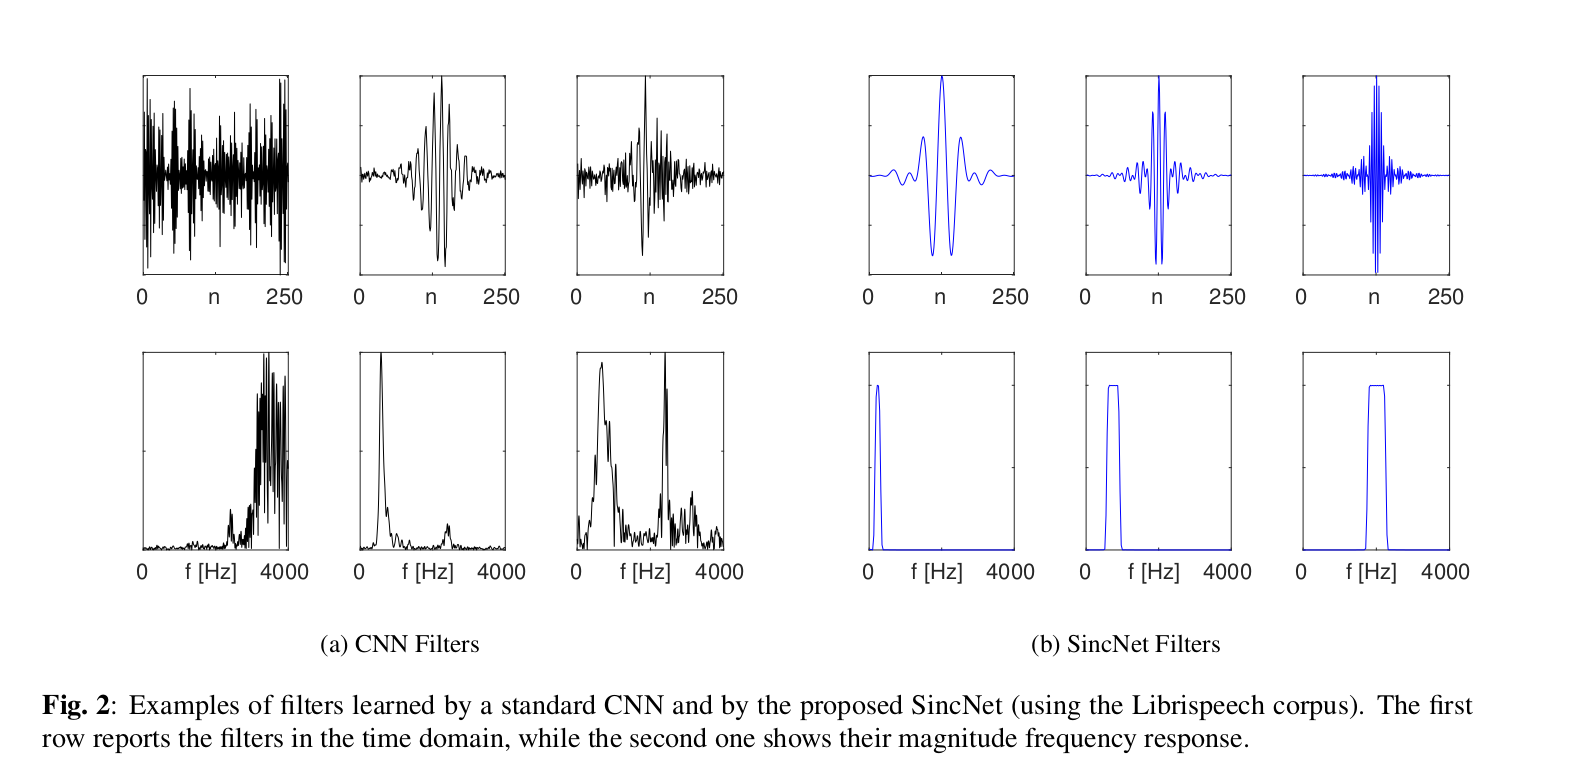
\includegraphics[width=1\textwidth]{images/cnn_filters_sincnet_filters.png}
		\caption{Ví dụ về các bộ lọc được học bởi CNN tiêu chuẩn và bởi SincNet (sử dụng kho ngữ liệu Librispeech). Hàng đầu tiên thể hiện các bộ lọc trong miền thời gian, trong khi hàng thứ hai hiển thị phản hồi tần số cường độ của chúng.}
		\label{fig:writing-thesis}
	\end{figure}
	
	\subsection{3.3 Các công trình liên quan đến bài báo}
	Liệt kê danh sách các công trình liên quan đến bài báo
	\textbf{Một số công trình trước đây khai thác đặc trưng cường độ phổ:}
	\begin{itemize}
		\item C. Zhang, K. Koishida, and J. Hansen, “Textindependent speaker verification based on triplet convolutional neural network embeddings,” IEEE/ACM Trans. Audio, Speech and Lang. Proc., vol. 26, no. 9,
		pp. 1633–1644, 2018.
		
		\item G. Bhattacharya, J. Alam, and P. Kenny, “Deep speaker
		embeddings for short-duration speaker verification,” in
		Proc. of Interspeech, 2017, pp. 1517–1521.
		
		\item A. Nagrani, J. S. Chung, and A. Zisserman, “Voxceleb:
		a large-scale speaker identification dataset,” in Proc. of
		Interspech, 2017.
		
		\item T. N. Sainath, B. Kingsbury, A. R. Mohamed, and
		B. Ramabhadran, “Learning filter banks within a deep
		neural network framework,” in Proc. of ASRU, 2013,
		pp. 297–302
		
		\item H. Yu, Z. H. Tan, Y. Zhang, Z. Ma, and J. Guo, “DNN
		Filter Bank Cepstral Coefficients for Spoofing Detection,” IEEE Access, vol. 5, pp. 4779–4787, 2017.
		
		\item H. Seki, K. Yamamoto, and S. Nakagawa, “A deep
		neural network integrated with filterbank learning for
		speech recognition,” in Proc. of ICASSP, 2017, pp.
		5480–5484.
	\end{itemize}
	\textbf{Các công trình tiếp cận bằng cách Học dựa vào sóng âm thô:}
	\begin{itemize}
		\item D. Palaz, M. Magimai-Doss, and R. Collobert, “Analysis of CNN-based speech recognition system using raw
		speech as input,” in Proc. of Interspeech, 2015.
		
		\item T. N. Sainath, R. J. Weiss, A. W. Senior, K. W. Wilson,
		and O. Vinyals, “Learning the speech front-end with raw
		waveform CLDNNs,” in Proc. of Interspeech, 2015.
		
		\item Y. Hoshen, R. Weiss, and K. W. Wilson, “Speech acoustic modeling from raw multichannel waveforms,” in
		Proc. of ICASSP, 2015.
		
		\item T. N. Sainath, R. J. Weiss, K. W. Wilson, A. Narayanan,
		M. Bacchiani, and A. Senior, “Speaker localization and
		microphone spacing invariant acoustic modeling from
		raw multichannel waveforms,” in Proc. of ASRU, 2015.
		
		\item Z. Tuske, P. Golik, R. Schl ¨ uter, and H. Ney, “Acous- ¨
		tic modeling with deep neural networks using raw time
		signal for LVCSR,” in Proc. of Interspeech, 2014.
	\end{itemize}

	\textbf{Trong các tác vụ}
	\begin{itemize}
		\item \textbf{Cảm xúc}
		\begin{itemize}
			\item G. Trigeorgis, F. Ringeval, R. Brueckner, E. Marchi,
			M. A. Nicolaou, B. Schuller, and S. Zafeiriou, “Adieu
			features? end-to-end speech emotion recognition using
			a deep convolutional recurrent network,” in Proc. of
			ICASSP, 2016, pp. 5200–5204.
		\end{itemize}
		\item \textbf{Nhận dạng người nói}
		\begin{itemize}
			\item H. Muckenhirn, M. Magimai-Doss, and S. Marcel, “Towards directly modeling raw speech signal for speaker
			verification using CNNs,” in Proc. of ICASSP, 2018.
		\end{itemize}
		\item \textbf{Phát hiện mạo danh}
		\begin{itemize}
			\item H. Dinkel, N. Chen, Y. Qian, and K. Yu, “End-toend spoofing detection with raw waveform CLDNNS,”
			Proc. of ICASSP, pp. 4860–4864, 2017.
		\end{itemize}
		\item \textbf{Tổng hợp giọng nói}
		\begin{itemize}
			\item A. van den Oord, S. Dieleman, H. Zen, K. Simonyan,
			O. Vinyals, A. Graves, N. Kalchbrenner, A. Senior, and
			K. Kavukcuoglu, “Wavenet: A generative model for raw
			audio,” in Arxiv, 2016.
			\item S. Mehri, K. Kumar, I. Gulrajani, R. Kumar, S. Jain,
			J. Sotelo, A. C. Courville, and Y. Bengio, “Samplernn:
			An unconditional end-to-end neural audio generation
			model,” CoRR, vol. abs/1612.07837, 2016.
		\end{itemize}
	\end{itemize}
	
	\subsection{3.4 Xây dựng mô hình}
	
	\subsubsection{3.4.1 Kho dữ liệu}
	\qquad Trong bài báo này, nhóm tác giả sử dụng hai tập ngữ liệu khá lớn đó là \textbf{TIMIT} (TIMIT Acoustic-Phonetic Continuous Speech Corpus) và \textbf{LibriSpeech}
	
	Với \textbf{TIMIT}, ta có một kho ngữ liệu với 462 người nói, các khoảng không phải lời nói ở đầu và cuối mỗi câu đã bị xóa, những tập tin về nội dung câu nói của TIMIT cũng được loại bỏ. Sau khi tinh chỉnh toàn bộ dữ liệu, tác giả dùng 5 câu nói của mỗi người nói để huấn luyện, 3 câu nói của mỗi người nói dùng để kiểm tra.
	
	Với tập ngữ liệu \textbf{LibriSpeech}, những phần với độ im lặng bên trong kéo dài hơn 125 ms được chia thành nhiều phần nhỏ. Việc chia tập huấn luyện (training set), tập kiểm tra (testing set) là ngẫu nhiên bằng cách chọn 12-15 giây dữ liệu huấn luyện của mỗi người nói và các câu kiểm tra kéo dài từ 2-6 giây. 
	
	\subsubsection{3.4.2 Xây dựng mô hình SincNet}
	\qquad Các sóng của mỗi câu nói được cắt thành những chunks khoảng 200ms (trong đó có 10 ms overlap) để có thể đưa vào mạng SincNet.
	
	Lớp input thực hiện hàm sinc dựa trên tích chập (convolutional) như đã nói ở phần mô tả kiến trúc mạng SincNet. Với thông số, 80 filters, mỗi filter có kích thước $L = 251$, dùng LayerNorm cho cả input và output,không dùng BatchNorm, activation LeakyReLU, không DropOut.
		
	Sau đó, kiến trúc sử dụng 2 CNNs chuẩn với 60 filters có kích thước $L = 5$, dùng LayerNorm cho cả input và output, không dùng BatchNorm, activation LeakyReLU, không DropOut.
	
	Kế tiếp là 3 lớp fully-connected layer - Multi Layer Perceptron (MLP), 2048 node, dùng LayerNorm cho input, dùng BatchNorm cho output, activation LeakyReLU, không DropOut.
	
	Lớp output, Multi Layer Perceptron (MLP), 462 class\_lay với TMIT hoặc class\_lay= 2484 với LibrisSpeech, không dùng LayerNorm hay BatchNorm, activation Softmax, không DropOut.
	
	Quá trình huấn luyện dùng RMSprop optimizer với learning\_rate $lr = 0.001, \alpha = 0.95, \epsilon = 10^{-7}$, minibatches\_size = 128
	
	Với hệ thống xác minh người nói, kế thừa từ \textbf{speaker-id neural networks} với hai cách tiếp cận cài đặt. Thứ nhất, chúng ta xem xét \textbf{d-vector framework}, dựa vào đầu ra của lớp ẩn cuối cùng và tính toán khoảng cách cosin giữa các \textbf{d-vectors} thử nghiệm và mẫu cần kiểm thử. Cách thay thế thứ hai (được biểu thị ở phần sau là \textbf{DNN-class}), hệ thống xác minh người nói có thể trực tiếp lấy điểm sau \textbf{softmax} tương ứng với danh tính được xác minh.
	
	\subsubsection{3.4.3 So sánh SincNet với các kiến trúc khác}
	Để so sánh SincNet với các hệ thống khác, trong bài báo nhóm tác giả đã đề xuất sự so sánh, cụ thể như sau:
	\begin{itemize}
		\item Thứ nhất, xem xét một kiến trúc CNN đầu vào là sóng thô (raw waveform), nhìn chung kiến trúc này không khác gì SincNet, nhưng thay vì dùng các hàm sinc trên tích chập, nó sẽ dùng một filter bình thường.
		\item Thứ hai, để so sánh với một số phương pháp xử lý đặc trưng thủ công phổ thông như FBANK, MFCC. Nhóm tác giả đề xuất cách so sánh như sau: tính toán 39 MFCCs (13 static + $\Delta$ + $\Delta\Delta$) và 40 \textbf{FBANKs} sử dụng \textbf{Kaldi toolkit}. Những đặc trưng sẽ được tính toán mỗi 25 ms trong đó overlap 10 ms, trong một cửa sổ (windows) xấp xỉ khoảng 200 ms. Mục đích của việc này nhằm mục đích tạo ra một tình huống gần như tương tự khi dùng một neural network). Một CNN được dùng cho đặc trưng \textbf{FBANKs} trong khi đó một \textbf{Multi-Layer Perceptron} (MLP) dùng cho MFCC. FBANK network dùng \textbf{Layer normalization}, MFCC Network sử dụng \textbf{Batch normalizaton}, các \textbf{hyper-parameters} cũng sẽ được điều chỉnh sao cho hợp lý nhất.
		\item Với tác vụ thử nghiệm xác minh người nói, nhóm tác giả cũng đề xuất một đối sánh với \textbf{i-vectors}. Hệ thống \textbf{i-vectors} được cài đặt với \textbf{SIDEKIT toolkit}. Các mô hình GMM-UBM, Total Variability matrix, Probabilistic Linear Discriminant Analysis (PLDA) cũng đã được huấn luyện trên tập LibriSpeech. GMM-UBM được tạo thành từ 2048 Gaussians, hạng của ma trận TV và ma trận giọng nói riêng (eigenvoice cũng tương tự như eigenvector) là 400. Giai đoạn đăng ký và kiểm tra được tiến hành trên Librispeech bằng cách sử dụng cùng một bộ phân đoạn giọng nói được sử dụng cho các thử nghiệm DNNs.
	\end{itemize}
	
	\subsection{3.5 Các kết quả}
	
	\subsubsection{3.5.1 Phân tích các bộ lọc}
	\begin{figure}[H]
		\centering
		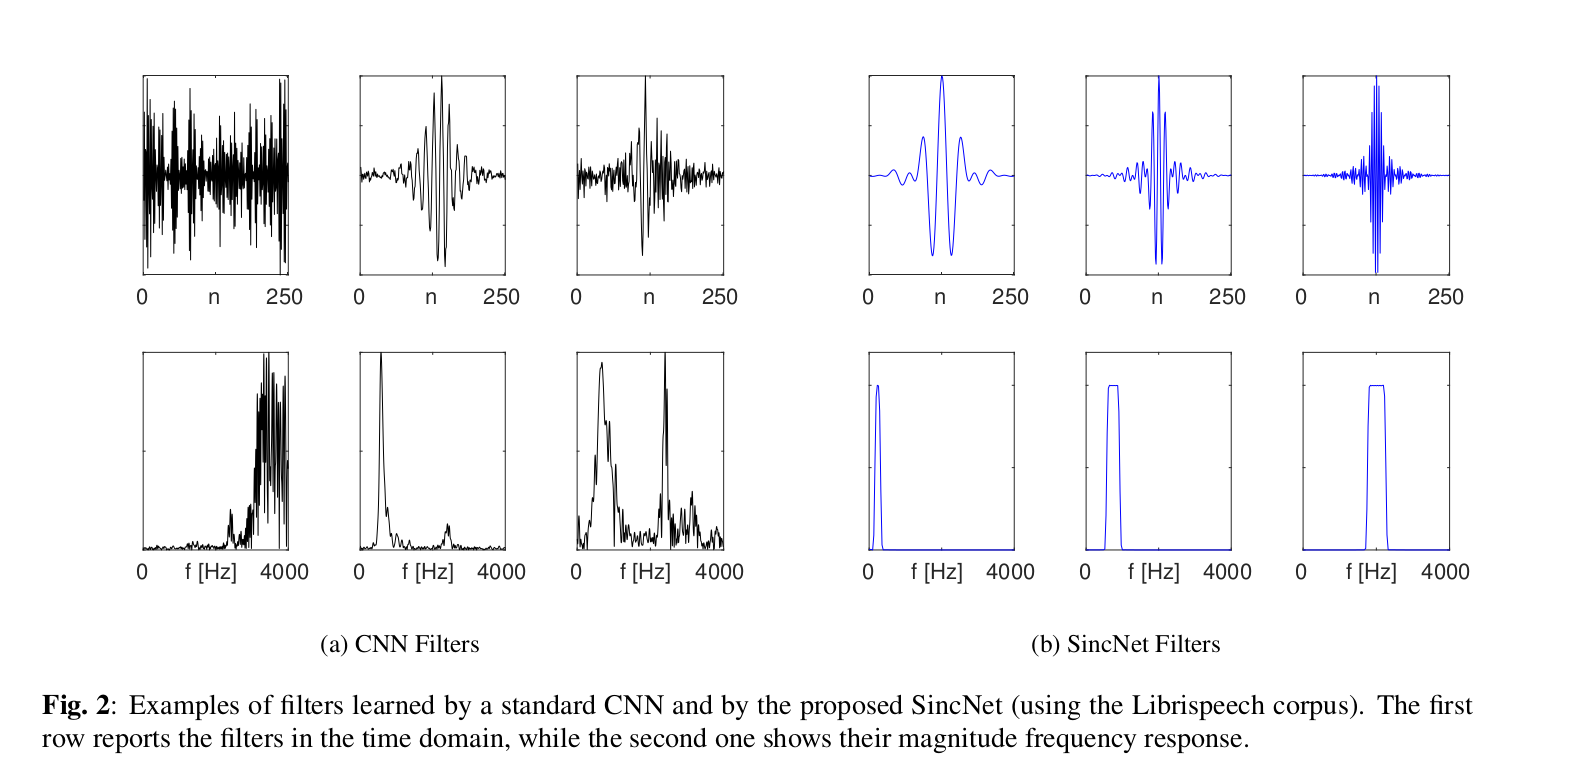
\includegraphics[width=1\textwidth]{images/cnn_filters_sincnet_filters.png}
		\caption{Ví dụ về các bộ lọc được học bởi CNN tiêu chuẩn và bởi SincNet (sử dụng kho ngữ liệu Librispeech). Hàng đầu tiên thể hiện các bộ lọc trong miền thời gian, trong khi hàng thứ hai hiển thị phản hồi tần số cường độ của chúng.}
		\label{fig:writing-thesis}
	\end{figure}
	Hình bên trên là sự so sánh mà nhóm tác giả đã dẫn chứng trong bài báo về cách mà một CNN (hình a) và SincNet (hình b) học từ filter như thế nào. Đây là những kết quả thực hiện trên tập dữ liệu LibriSpeech, tần số phản hồi biểu diễn từ 0 đến 4kHz. Ở trường hợp CNN, nó không luôn luôn học từ filter, bằng chứng là những đường tần số không đều, chứa đầy nhiễu (filter đầu tiên). Trong khi đó, với SincNet Filters, ta thu được những hình ảnh đều đặng hơn về tần số, có sự "đối xứng" xuất hiện ở miền thời gian, hình dạng trên miền tần số giống như hình chữ nhật, nó dường như có ý nghĩa hơn.
	
	\begin{figure}[H]
		\centering
		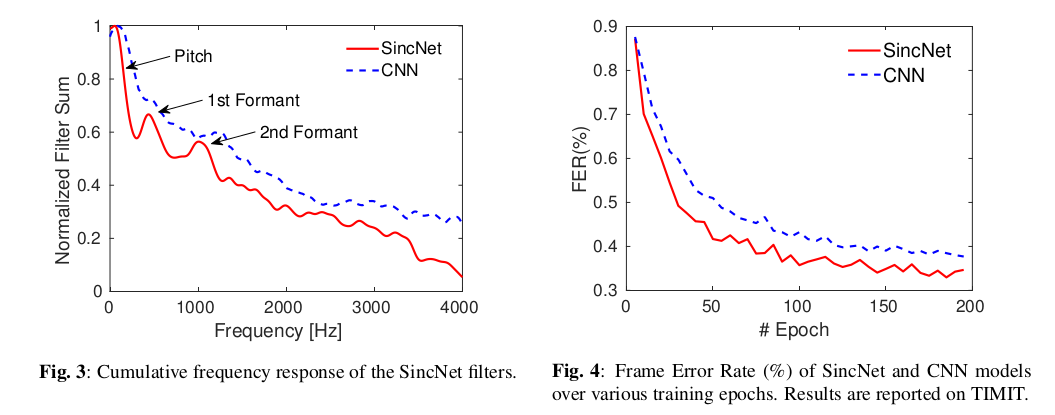
\includegraphics[width=1\textwidth]{images/filter_analysis.png}
		\caption{Bảng kết quả SicNet trong tác vụ nhận dạng giọng nói - SI}
		\label{fig:writing-thesis}
	\end{figure}
	Ngoài việc kiểm tra định tính, điều quan trọng là phải làm nổi bật dải tần nào được bao phủ bởi các bộ lọc đã học. 
	
	Hình 3 cho thấy đáp ứng tần số tích lũy của các bộ lọc được học bởi SincNet và CNN. Điều thú vị là có \textbf{ba đỉnh chính nổi bật} rõ ràng với biểu đồ SincNet (xem đường màu đỏ trong hình). \textbf{Âm đầu tiên tương ứng với vùng cao độ} (cao độ trung bình là 133 Hz đối với nam và 234 đối với nữ). \textbf{Đỉnh thứ hai (nằm gần đúng ở tần số 500 Hz)} chủ yếu thu nhận các định dạng đầu tiên, có giá trị trung bình so với các nguyên âm tiếng Anh khác nhau thực sự là 500 Hz. Cuối cùng, \textbf{đỉnh thứ ba (dao động từ 900 đến 1400 Hz)} nắm bắt một số định dạng thứ hai quan trọng, chẳng hạn như định dạng thứ hai của nguyên âm /a/ có vị trí trung bình ở tần số 1100 Hz. Cấu hình tập các bộ lọc này chỉ ra rằng SincNet đã điều chỉnh thành công các đặc điểm của nó để giải quyết vấn đề nhận dạng người nói. Ngược lại, với \textbf{CNN không thể hiện một mô hình có ý nghĩa như vậy}: các bộ lọc CNN có xu hướng tập trung chính xác vào phần dưới của phổ tần số, nhưng các đỉnh được điều chỉnh trên các công thức thứ nhất và thứ hai không xuất hiện rõ ràng. Như mọi người có thể quan sát từ Hình 3, đường cong CNN đứng trên đường SincNet. Trên thực tế, SincNet học từ các bộ lọc trung bình chọn lọc hơn các bộ lọc của CNN, có thể nắm bắt đặc trưng có dải tần hẹp tốt hơn.

	\subsubsection{3.5.2 Tác vụ nhận dạng giọng nói - Speaker Identification}
	\qquad Như đã dẫn chứng ở trên, ở hình 4 trong bài báo, cho thấy learning curves của SincNet so với CNN. Ta có thể thấy rằng, Frame Error Rate giảm thực sự nhanh khi dùng SincNet. Hơn nữa, SincNet hội tụ với hiệu suất tốt hơn với FER $33.0\%$ so với FER $37.7\%$ của CNN
	
	\begin{figure}[H]
		\centering
		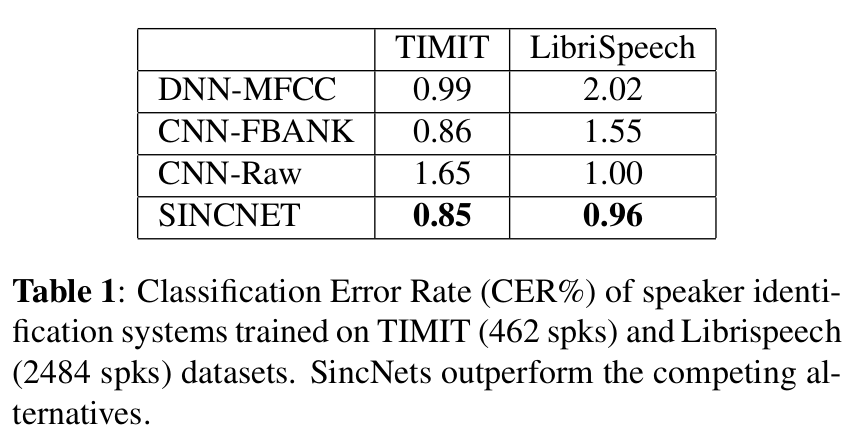
\includegraphics[width=0.65\textwidth]{images/performance_speaker_identification.png}
		\caption{Bảng kết quả SicNet trong tác vụ nhận dạng giọng nói - SI}
		\label{fig:writing-thesis}
	\end{figure}
	Bảng trên đây là một bảng báo cáo về tỉ lệ phân lớp lỗi (\textbf{Classification Error Rates - CER\%}), khi thực nghiệm SincNet cùng với số kỹ thuật khác như \textbf{DNN-MFCC, CNN-FBANK, CNN-Raw} trên hai tập dữ liệu \textbf{TIMIT} và \textbf{LibriSpeech}. Nhìn chung, SincNet luôn dẫn đầu về độ lỗi tốt (có độ lỗi thấp nhất). Độ lỗi của \textbf{CNN-Raw} thật sự lớn khi tiến hành với tập TIMIT, điều này cho thấy S\textbf{SincNet} của chúng ta hoạt động tốt ngay cả khi có không lớn dữ liệu huấn luyện có sẵn. Khi huấn luyện với \textbf{LibriSpeech}, độ lỗi \textbf{CNN-Raw} giảm xuống, chúng ta có 4\% độ lỗi được giảm xuống, điều này cho thấy tốc độ hội tụ của SincNet cải thiện rõ ràng (1200 và 1800 epochs). Với \textbf{DNN-MFCC, CNN-FBANK}, hai kỹ thuật này hoạt động tốt trên \textbf{TIMIT} (vì đơn giản là \textbf{TIMIT} không lớn cho lắm như \textbf{LibriSpeech}), khi sang \textbf{LibriSpeech}, chúng có vẻ mất đi tính ổn định, độ lỗi cao lên.
	
	\subsubsection{3.5.3 Tác vụ xác minh giọng nói - Speaker Verification}
	Thử nghiệm cuối cùng mà nhóm tác giả trình bày ở trong bài báo là tác vụ \textbf{xác minh giọng nói - Speaker Verification}. Bảng dưới đây, được trích ra trong bài báo, báo cáo về chỉ số \textbf{Equal Error Rate} (EER\%) khi thực nghiệm trên tập \textbf{LibriSpeech}. 
	\begin{figure}[H]
		\centering
		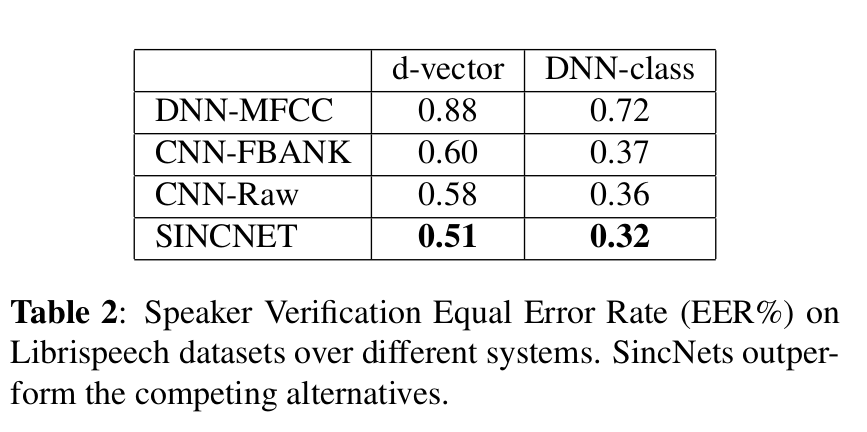
\includegraphics[width=0.65\textwidth]{images/performance_speaker_verification.png}
		\caption{Bảng kết quả SicNet trong tác vụ xác minh giọng nói - SV}
		\label{fig:writing-thesis}
	\end{figure}

	Tất cả các mô hình DNN đều cho thấy hiệu suất đầy hứa hẹn, \textbf{các chỉ EER thấp hơn 1\% trong mọi trường hợp}. Bảng cũng cho thấy rằng \textbf{SincNet lại một lần nữa hoạt động tốt hơn các mô hình khác}, cho thấy sự cải thiện hiệu suất tương đối khoảng \textbf{11\% so với mô hình CNN}. Các mô hình lớp DNN hoạt động tốt hơn đáng kể so với các \textbf{d-vector}. Bất chấp hiệu quả của cách tiếp cận sau này, một mô hình DNN mới phải được huấn luyện (hoặc tinh chỉnh) cho mỗi người nói mới được thêm vào nhóm. Điều này làm cho cách tiếp cận này hoạt động tốt hơn, nhưng kém linh hoạt hơn so với \textbf{d-vector}.
	
	Để hoàn thiện hơn, nhóm tác giả cũng tiến hành các thí nghiệm khác với các \textbf{i-vector} tiêu chuẩn. Tuy nhiên so sánh chi tiết với kỹ thuật này nằm ngoài phạm vi của bài báo nên nhóm tác giả chỉ nêu ra những điểm đáng chú ý nhất trong kết quả. Hệ thống \textbf{i-vector} tốt nhất của nhóm tác giả đạt được \textbf{EER = 1,1\%}, \textbf{khá xa so với những gì đạt được với hệ thống DNN}. Tài liệu nổi tiếng rằng \textbf{i-vector} cung cấp hiệu suất cạnh tranh khi sử dụng nhiều dữ liệu huấn luyện hơn cho mỗi người nói và khi các câu kiểm tra dài hơn được sử dụng. Trong các điều kiện thách thức phải đối mặt trong công việc này, mạng neural đạt được khả năng tổng quát hóa tốt hơn.

	\section{4. Thực nghiệm của nhóm}
	\subsection{4.1 Phương pháp giải quyết vấn đề}
	Cài đặt mô hình Nhận dạng Người nói và đánh giá nó với tiếng Việt và tiếng Anh với SincNet.
	Các tác vụ thành phần của mô hình: Identification (Định danh) và Verification (Xác minh)
	
	\subsection{4.2 Tập dữ liệu thực nghiệm}
	\qquad \textbf{Tiếng Anh} Sử dụng hai tập dữ liệu đã được đề cập trong bài báo

	Với \textbf{TIMIT}, ta có một kho ngữ liệu với 462 người nói, các khoảng không phải lời nói ở đầu và cuối mỗi câu đã bị xóa, những tập tin về nội dung câu nói của TIMIT cũng được loại bỏ. Sau khi tinh chỉnh toàn bộ dữ liệu, tác giả dùng 5 câu nói của mỗi người nói để huấn luyện, 3 câu nói của mỗi người nói dùng để kiểm tra.
	
	Với tập ngữ liệu \textbf{LibriSpeech}, những phần với độ im lặng bên trong kéo dài hơn 125 ms được chia thành nhiều phần nhỏ. Việc chia tập huấn luyện (training set), tập kiểm tra (testing set) là ngẫu nhiên bằng cách chọn 12-15 giây dữ liệu huấn luyện của mỗi người nói và các câu kiểm tra kéo dài từ 2-6 giây. 
	
	\textbf{Tiếng Việt} Sử dụng tập dữ liệu Son et al. Dataset
	
	Nguồn dữ liệu từ bài báo Vietnamese Speaker Authentication Using Deep Models
	\begin{itemize}
		\item Dung lượng của tập dữ liệu: 535 MB
		\item Số mẫu trong tập dữ liệu: 400 mẫu
		\item Bộ dữ liệu gồm: hai tập  Men và Women, mỗi tập con chứa 10 thư mục người nói. Mỗi thư mục người nói chứa 20 đoạn ghi âm, chia ra Long và Short (mỗi loại 10 đoạn) 
		\item Nội dung câu nói
		\begin{itemize}
			\item Câu ngắn: “Tôi là sinh viên chuyên ngành công nghệ thông tin"
			\item Câu dài: "Tôi là sinh viên Học viện Công nghệ Bưu chính Viễn thông, chương trình đào tạo khá nặng đòi hỏi sinh viên phải học tập và nghiên cứu rất nhiều nhưng tôi tự hào vì đó là ngành đã và đang làm thay đổi cuộc sống xã hội loài người".
		\end{itemize}
		\item Điểm hạn chế: Bộ dữ liệu có kích thước khá nhỏ
	\end{itemize}
	
	Ngoài ra, nhóm tự ghi âm thêm dữ liệu với độ dài tương tự như tập này.
	\subsection{4.3 Thử nghiệm thực nghiệm với tiếng Việt}
	\subsubsection{4.3.1 Thu thập - Tiền xử lý dữ liệu, gán nhãn}
	
	\subsubsection{4.3.2 Phân chia tập dữ liệu}
	
	\subsubsection{4.3.3 Điều chỉnh thông số và huấn luyện}
	
	\subsubsection{4.3.4 Đánh giá}
	
	\subsection{4.3 Thử nghiệm thực nghiệm với tiếng Anh với tập TIMIT}
	\subsubsection{4.3.1 Tải và điều chỉnh dữ liệu}
	
	\subsubsection{4.3.2 Huấn luyện mô hình}
	
	\subsubsection{4.3.3 Đánh giá mô hình}
	
	\subsubsection{4.3.4 So sánh với kết quả có trong bài báo}
	
	\subsection{4.3 Thử nghiệm thực nghiệm với tiếng Anh với tập LibrisSpeech}
	\subsubsection{4.3.1 Tải và điều chỉnh dữ liệu}
	
	\subsubsection{4.3.2 Huấn luyện mô hình}
	
	\subsubsection{4.3.3 Đánh giá mô hình}
	
	\subsubsection{4.3.4 So sánh với kết quả có trong bài báo}
	
	\section{5. Kế hoạch thực hiện}
	
	\subsection{5.1 Timeline}
	\scalebox{1}{
		\begin{tabular}{r |@{\foo} l}
			
			29/03 - 04/04 & Tiếp nhận đồ án, phân công công việc\\
			05/04 - 11/04 & Đọc source code mẫu từ Github, trình bày những gì tìm hiểu được\\
			12/04 - 18/04 & Chạy thử source code mẫu từ Github, trình bày những gì tìm hiểu được\\
			19/04 - 25/04 & Trình bày những gì tìm hiểu được, phân công làm slides, quay video trình bày đồ án\\
			26/04 - 02/05 & Thu thập dữ liệu, tiền xử lý dữ liệu\\
			03/05 - 09/05 & Tinh chỉnh source code, chạy thử mô hình\\
			10/05 - 16/05 & Huấn luyện mô hình\\
			17/05 - 23/05 & Phân công làm slides, quay video trình bày đồ án\\
			24/05 - 30/05 & *Dự phòng\\
			31/05 - 06/06 & *Dự phòng\\
			
		\end{tabular}
	}

	\subsection{5.2 Vai trò của các thành viên}
	
	\begin{center}
		\begin{tabular}{ | c | c | c | c | c |}\hline
			STT	& MSSV & Họ tên đầy đủ & Email liên lạc & Vai trò\T\B\\\hline
			1 & 18120009 & Vương Gia Bảo & 18120009@student.hcmus.edu.vn  & Thành viên \T\B\\ \hline
			2 & 18120045 & Ngô Xuân Kiên & 18120045@student.hcmus.edu.vn & Thành viên\T\B\\ \hline
			3 & 18120061 & Lê Nhựt Nam & 18120061@student.hcmus.edu.vn & Nhóm trưởng \T\B\\ \hline
			4 & 18120167 & Nguyễn Viết Dũng &  18120167@student.hcmus.edu.vn & Thành viên \T\B\\ \hline
		\end{tabular}
	\end{center}

	\subsection{5.3 Phân công công việc}
	\begin{center}
		\begin{tabular}{ | l | l | l | p{5cm} | p{3cm} |}
			\hline
			STT & MSSV & Họ tên & Nội dung công việc & Mức độ hoàn thành công việc  \T\B\\ \hline
			1 & 18120009 & Vương Gia Bảo & Thu thập dữ liệu, đọc hiểu source, báo cáo Introduction Paper &  100\%\T\B\\ \hline
			2 & 18120045 & Ngô Xuân Kiên & Thu thập dữ liệu, đọc hiểu source, báo cáo Related Work Paper & 100\%\T\B \\ \hline
			3 & 18120061 & Lê Nhựt Nam & Thu thập dữ liệu, đọc hiểu source, báo cáo, SincNet Architecture, Slides thuyết trình, Midterm Report & 100\%\T\B \\ \hline
			4 & 18120167 & Nguyễn Viết Dũng &  Thu thập dữ liệu, đọc hiểu source, báo cáo experimental setup Paper & 100\%\T\B \\ \hline
		\end{tabular}
	\end{center}
	\nocite{*}
	\bibliography{references}\newpage\cleardoublepage
	\bibliographystyle{plain}
	
\end{document}
